\documentclass[runningheads]{llncs}

\usepackage{fontspec}
\setmainfont{Times New Roman}
\setsansfont{Arial}
\setmonofont{Consolas}
\usepackage{amsmath,amssymb}
\usepackage{booktabs}
\usepackage{tabularx}
\usepackage{ragged2e}
\usepackage{makecell}
\usepackage{multirow}
\usepackage{graphicx}
\usepackage{xcolor}
\usepackage{subcaption}
\usepackage{float}
\usepackage[hidelinks]{hyperref}
\usepackage{cleveref}

\newcommand{\Epre}{\ensuremath{E_{\text{pre}}}}
\newcommand{\Esim}{\ensuremath{E_{\text{sim}}}}
\newcommand{\KC}{thành phần kiến thức}
\newcommand{\KCs}{thành phần kiến thức}
\newcommand{\DDR}{\textsc{DDR}}

\begin{document}

\title{Xây dựng đồ thị khái niệm kiểm soát rò rỉ và giao thức chẩn đoán cold-start cho Knowledge Tracing}
\titlerunning{Giao thức đồ thị kiểm soát rò rỉ cho KT}

\author{Dao Minh Tuan\inst{1} \and
Nguyen Tien Duong\inst{1} \and
Nguyen Khanh Trinh\inst{1} \and
Nguyen Van Hau\inst{1} \and
Le Hoang Son\inst{2}}
\authorrunning{D.~M. Tuan et al.}

\institute{Hung Yen University of Technology and Education, Hung Yen, Vietnam\\
\email{tuan.ymc@gmail.com}
\and
VNU Information Technology Institute, Vietnam National University,\\
144 Xuan Thuy Street, Cau Giay Ward, Ha Noi, Vietnam}

\maketitle

\begin{abstract}
Các mô hình Knowledge Tracing (KT) ngày càng sử dụng đồ thị khái niệm để mô tả quan hệ giữa các kỹ năng hoặc bài tập. Tuy nhiên, nếu đồ thị được suy luận từ toàn bộ nhật ký tương tác trước khi chia train/validation/test, thông tin từ người học ở tập kiểm tra có thể đi vào mô hình qua cạnh đồ thị. Bài báo này trình bày một giao thức xây dựng và kiểm toán đồ thị \KC{} có kiểm soát rò rỉ cho KT. Giao thức áp dụng chia tách theo người học, suy luận cạnh chỉ từ tập train, kiểm tra DAG kèm tỉa chu trình, chẩn đoán cold-start theo tần suất \KC{}, và chỉ số DAG Disruption Rate (\DDR{}) để đo độ nhạy của cấu trúc đồ thị trước các phép tăng cường.

Giao thức được thực nghiệm trên Junyi Academy, ASSISTments~2012, XES3G5M và hai bộ synthetic C2/C5. Kết quả kiểm toán cho thấy tất cả đồ thị tiên quyết train-only đều có thể đưa về DAG sau bước tỉa chu trình. Trên Junyi, nơi có chú giải tiên quyết do chuyên gia xây dựng, đồ thị suy luận từ hành vi và đồ thị chuyên gia có tương quan cao ở mức nút (Jaccard xấp xỉ $0.63$) nhưng yếu hơn ở mức cạnh (F1 xấp xỉ $0.18$ tại $K=|\text{expert}|$), cho thấy hai nguồn tín hiệu liên quan nhưng không thay thế trực tiếp cho nhau. Với đánh giá kiểm soát rò rỉ, GKT không nhất quán vượt \textit{simpleKT}/AKT trên ASSISTments và XES3G5M. Các hàng GIKT native được tạm loại khỏi diễn giải vì cache cũ có lỗi lệch chỉ số gây rò đáp án hiện tại, cần chạy lại sau khi sửa. Bài báo được định vị là một giao thức và tài nguyên tái lập cho KT tăng cường đồ thị, không phải một mô hình KT mới.
\keywords{Knowledge tracing \and Đồ thị khái niệm \and Kiểm soát rò rỉ \and DAG \and Cold-start \and Tái lập}
\end{abstract}

\section{Giới thiệu}
Knowledge Tracing dự đoán trạng thái nắm vững kiến thức của người học từ chuỗi tương tác học tập, hỗ trợ hệ thống luyện tập thích nghi, khuyến nghị bài học và đánh giá năng lực. Các mô hình hiện đại đi từ Bayesian Knowledge Tracing~\cite{corbett1995bkt}, Deep Knowledge Tracing~\cite{piech2015dkt}, đến các kiến trúc attention như AKT và simpleKT~\cite{ghosh2020akt,liu2023simplekt}. Một hướng phát triển quan trọng là bổ sung cấu trúc đồ thị giữa các \KCs{} hoặc bài tập, ví dụ GKT~\cite{nakagawa2019gkt}, GIKT~\cite{yang2021gikt}, SKT~\cite{tong2020skt}, DyGKT và DGEKT.

Vấn đề của các đồ thị suy luận từ log là \emph{nguồn gốc cạnh}. Nếu cạnh được xây dựng từ toàn bộ log rồi mới chia tập dữ liệu, cạnh đó có thể mã hóa chuyển tiếp hoặc đồng xuất hiện từ người học ở validation/test. Khi đó mô hình không nhìn trực tiếp nhãn kiểm tra, nhưng đã nhận thông tin cấu trúc có nguồn gốc từ tập kiểm tra. Vì vậy, so sánh giữa mô hình đồ thị và mô hình chuỗi có thể bị lệch bởi quy trình tiền xử lý thay vì do bản thân kiến trúc.

Bài báo này đề xuất một giao thức nhằm biến nguồn gốc cạnh thành một đối tượng kiểm toán rõ ràng. Giao thức yêu cầu mỗi fold tự tạo đồ thị từ người học train, ghi provenance cho từng cạnh, kiểm tra chu trình, báo cáo rò rỉ trực tiếp, đo ảnh hưởng của việc dùng full-log graph so với train-only graph, và tách kết quả theo tần suất \KC{} để quan sát cold-start.

\paragraph{Đóng góp.}
Bản tiếng Việt này tóm lược cùng bộ kết quả với bản LNNS tiếng Anh hiện tại:
\begin{itemize}
  \item Giao thức xây dựng \Epre{} và \Esim{} theo fold, chỉ dùng tập train, có kiểm toán rò rỉ và kiểm toán DAG.
  \item Chỉ số \DDR{} để đo mức phá vỡ cấu trúc tiên quyết khi áp dụng các phép tăng cường đồ thị.
  \item Chẩn đoán cold-start theo strata tần suất \KC{} thay vì chỉ báo cáo AUC tổng hợp.
  \item Đối chiếu Junyi với đồ thị chuyên gia để phân biệt tín hiệu hành vi và tín hiệu sư phạm.
  \item Kết quả baseline cập nhật: ASSISTments có 3-fold learner CV; Junyi đã bổ sung SKT từ cache; XES3G5M và các bộ synthetic vẫn dùng fold~0 trong bản phát hành này.
\end{itemize}

\section{Giao thức đề xuất}
\subsection{Thiết lập chia dữ liệu}
Với mỗi dataset $D$, giao thức chia người học thành train/validation/test theo tỉ lệ $(0.7,0.1,0.2)$. Mọi cạnh đồ thị ở fold $f$ chỉ được suy luận từ tương tác của người học trong $\mathcal{F}_{\text{train}}^f$. Validation và test chỉ được dùng để đánh giá mô hình KT, không được dùng để đếm chuyển tiếp, đồng xuất hiện hoặc chuẩn hóa trọng số cạnh.

\subsection{Đồ thị tiên quyết và đồ thị tương tự}
Giao thức sinh hai loại quan hệ:
\begin{itemize}
  \item $\Epre$: cạnh có hướng biểu diễn quan hệ tiên quyết suy luận từ thứ tự tương tác trong tập train.
  \item $\Esim$: cạnh tương tự không hướng hoặc đối xứng, dựa trên mức chồng lấp KC/item khi dataset có đủ thông tin.
\end{itemize}
Sau khi lọc theo ngưỡng hỗ trợ, top-$k$ và giới hạn toàn cục $K$, đồ thị $\Epre$ được kiểm tra chu trình. Nếu có chu trình, pipeline loại cạnh có độ tin cậy thấp nhất trong chu trình cho đến khi đồ thị trở thành DAG. Cách làm này không khẳng định cạnh còn lại là ``đúng'' theo sư phạm, nhưng làm cho phép suy luận và kiểm toán có thể tái lập.

\subsection{Chỉ số kiểm toán}
Giao thức báo cáo bốn nhóm chỉ số:
\begin{itemize}
  \item \textbf{ECR flag}: chỉ báo rò rỉ cấu trúc do người học xuất hiện ở nhiều split. Giá trị $0$ xác nhận split rời nhau theo người học.
  \item \textbf{ECR overlap}: tỉ lệ mẫu cạnh hoặc transition cũng xuất hiện trong held-out. Chỉ số này có thể cao trên log dày đặc dù không vi phạm train-only.
  \item \textbf{EOC}: chuẩn Frobenius đo tương quan giữa khối lượng cạnh và outcome.
  \item \textbf{TBVR}: tỉ lệ vi phạm ranh giới thời gian trong train, dùng để kiểm tra mức trộn tín hiệu sớm/muộn trong chính tập train.
\end{itemize}

\section{Dữ liệu và thiết lập thực nghiệm}
Giao thức được chạy trên Junyi Academy, ASSISTments~2012, XES3G5M, Synthetic C2 và Synthetic C5. Junyi có chú giải tiên quyết do chuyên gia xây dựng, nhưng chú giải này không được dùng để tạo đồ thị ở nhánh chính; nó chỉ được dùng trong bước đối chiếu ground-truth. ASSISTments có Q-matrix nhưng không có đồ thị tiên quyết. XES3G5M có metadata phân cấp về KC; trong pipeline hiện tại, metadata này được chuyển thành ID KC ở mức chuỗi, còn cạnh tiên quyết vẫn được suy luận bằng cùng quy tắc train-only.

\begin{table}[t]
\centering
\footnotesize
\caption{Các dataset trong giao thức. Con số chi tiết được sinh bởi \texttt{results/tables/dataset\_stats.tex} trong bản tiếng Anh; bảng này tóm lược vai trò thực nghiệm.}
\label{tab:vi-datasets}
\begin{tabularx}{\textwidth}{@{}lXl@{}}
\toprule
Dataset & Vai trò trong kiểm toán & Ghi chú \\
\midrule
Junyi Academy & Benchmark công khai có expert prerequisite & Dùng để đối chiếu hành vi--chuyên gia \\
ASSISTments 2012 & Benchmark công khai có Q-matrix & Baseline đã có 3-fold learner CV \\
XES3G5M & Benchmark lớn, metadata KC phân cấp & Baseline fold~0 trong bản phát hành \\
Synthetic C2/C5 & Sanity corpora có cấu trúc nhỏ & Kiểm tra độ nhạy của ablation \\
\bottomrule
\end{tabularx}
\end{table}

\section{Kết quả kiểm toán đồ thị}
\subsection{Rò rỉ và DAG}
Trên các bản chạy phát hành, $\mathrm{ECR}^{\mathrm{flag}}=0$ cho mọi dataset, xác nhận không có người học xuất hiện đồng thời ở train/validation/test trong cùng fold. $\mathrm{ECR}^{\mathrm{overlap}}$ gần $1$ trên các log dày đặc vì mẫu chuyển tiếp lặp lại giữa các người học khác nhau; đây là overlap chẩn đoán, không phải vi phạm train-only.

Ở Junyi fold~0, suy luận train-only tạo $2{,}152$ cạnh ứng viên. Bước tỉa chu trình loại $1{,}013$ cạnh có độ tin cậy thấp, giữ lại $1{,}139$ cạnh acyclic trên $573$ nút. ASSISTments fold~0 có $386$ cạnh ứng viên, giữ $239$ cạnh sau tỉa; XES3G5M giữ $701$ trên $1{,}162$ cạnh ứng viên. Kết quả này cho thấy cycle pruning không phải bước trang trí: ngay cả khi chỉ dùng train, dữ liệu hành vi vẫn có thể tạo quan hệ hai chiều hoặc xung đột.

\begin{figure}[t]
\centering
\begin{subfigure}[t]{0.32\textwidth}
  \centering
  
\includegraphics[width=\linewidth]{results/figures/fig_kt_graph_junyi.pdf}
  \caption{Junyi}
\end{subfigure}
\hfill
\begin{subfigure}[t]{0.32\textwidth}
  \centering
  
\includegraphics[width=\linewidth]{results/figures/fig_kt_graph_assist2012.pdf}
  \caption{ASSISTments}
\end{subfigure}
\hfill
\begin{subfigure}[t]{0.32\textwidth}
  \centering
  
\includegraphics[width=\linewidth]{results/figures/fig_kt_graph_xes3g5m.pdf}
  \caption{XES3G5M}
\end{subfigure}
\caption{Minh họa các chuỗi tiên quyết có hỗ trợ cao sau kiểm toán DAG. Hình chỉ dùng để diễn giải, không dùng trong huấn luyện.}
\label{fig:vi-graphs}
\end{figure}

\subsection{DAG Disruption Rate}
\DDR{} đo tỉ lệ cạnh tiên quyết bị ảnh hưởng khi áp dụng phép tăng cường đồ thị. Bốn nhóm tăng cường tạo bốn chế độ cấu trúc khác nhau: mask thuộc tính gần như không đổi cấu trúc, drop cạnh phá vỡ gần tuyến tính theo xác suất, subgraph random-walk giữ kết nối tốt hơn, còn drop nút gây nhiễu mạnh nhất do mất toàn bộ cạnh kề. Kết quả này giúp phân biệt các phép tăng cường label-agnostic theo tác động cấu trúc, thay vì chỉ xem chúng như nhiễu ngẫu nhiên.

\begin{figure}[t]
\centering
\begin{subfigure}[t]{0.32\textwidth}
  \centering
  
\includegraphics[width=\linewidth]{results/figures/fig_ddr_junyi.pdf}
  \caption{Junyi}
\end{subfigure}
\hfill
\begin{subfigure}[t]{0.32\textwidth}
  \centering
  
\includegraphics[width=\linewidth]{results/figures/fig_ddr_assist2012.pdf}
  \caption{ASSISTments}
\end{subfigure}
\hfill
\begin{subfigure}[t]{0.32\textwidth}
  \centering
  
\includegraphics[width=\linewidth]{results/figures/fig_ddr_xes3g5m.pdf}
  \caption{XES3G5M}
\end{subfigure}
\caption{DAG Disruption Rate của các phép tăng cường đồ thị.}
\label{fig:vi-ddr}
\end{figure}

\section{Baseline KT}
\begin{table}[t]
\centering
\footnotesize
\caption{Baseline chẩn đoán cập nhật. ASSISTments là trung bình 3 fold; các dataset còn lại là fold~0 trong bản phát hành.}
\label{tab:vi-baseline}
\begin{tabular}{@{}llccc@{}}
\toprule
Dataset & Mô hình & AUC & ACC & NLL \\
\midrule
Junyi & \textit{simpleKT} & 0.989 & 0.962 & 0.093 \\
Junyi & SKT & 0.986 & 0.954 & 0.107 \\
Junyi & BKT & 0.779 & 0.847 & 0.377 \\
\midrule
ASSISTments & \textit{simpleKT} & 0.968 & 0.916 & 0.173 \\
ASSISTments & AKT & 0.968 & 0.916 & 0.175 \\
ASSISTments & GKT & 0.961 & 0.907 & 0.185 \\
ASSISTments & SKT & 0.953 & 0.898 & 0.198 \\
\midrule
XES3G5M & \textit{simpleKT} & 0.874 & 0.857 & 0.325 \\
XES3G5M & GKT & 0.835 & 0.842 & 0.365 \\
XES3G5M & SKT & 0.623 & 0.799 & 0.483 \\
\bottomrule
\end{tabular}
\end{table}

Trên ASSISTments, \textit{simpleKT}/AKT nằm quanh $0.968$ và GKT quanh $0.961$. Các số GIKT native cũ bị loại khỏi bảng vì lỗi alignment trong implementation đã làm mô hình nhìn thấy đáp án hiện tại; cần chạy lại trước khi diễn giải. Trên XES3G5M, GKT thấp hơn nhóm \textit{simpleKT}/AKT khoảng $0.039$ AUC; trên Junyi, SKT cache đạt $0.986$ nhưng các hàng GKT, GIKT, DyGKT, DGEKT chưa có trong bảng baseline chính do giới hạn bộ nhớ và thời gian chạy.

\begin{table}[t]
\centering
\footnotesize
\caption{Tóm tắt 3-fold learner CV trên ASSISTments. Wilcoxon có ít fold nên kém mạnh thống kê; bảng được giữ để minh bạch quy trình.}
\label{tab:vi-cv}
\begin{tabular}{@{}lcccc@{}}
\toprule
Mô hình & AUC & ACC & NLL & $p_{\text{W}}$ vs. \textit{simpleKT} \\
\midrule
\textit{simpleKT} & $0.968 \pm 0.000$ & $0.916 \pm 0.001$ & $0.173 \pm 0.001$ & --- \\
GKT & $0.961 \pm 0.001$ & $0.907 \pm 0.001$ & $0.185 \pm 0.001$ & 0.250 \\
GIKT & -- & -- & -- & cần chạy lại \\
SKT & $0.953 \pm 0.001$ & $0.898 \pm 0.001$ & $0.198 \pm 0.001$ & 0.250 \\
DyGKT & $0.952 \pm 0.001$ & $0.899 \pm 0.001$ & $0.200 \pm 0.002$ & 0.250 \\
\bottomrule
\end{tabular}
\end{table}

\section{Ablation train-only so với full-log}
Để kiểm tra giả thuyết rò rỉ, thí nghiệm ablation thay đồ thị train-only của từng fold bằng một đồ thị full-log suy luận từ toàn bộ bảng tương tác đã tiền xử lý, trong khi split người học và code đánh giá KT giữ nguyên. Nếu pooling full-log tạo lợi thế lớn, AUC/ACC của nhánh full-log sẽ tăng rõ rệt.

Kết quả phát hành cho thấy trên ASSISTments, XES3G5M và Junyi, $\Delta$AUC và $\Delta$ACC của mọi mô hình đồ thị làm tròn về $0.000$ ở ba chữ số thập phân. Synthetic C5 có dịch chuyển lớn nhất: GIKT tăng khoảng $0.004$ AUC, còn GKT giảm khoảng $0.006$ AUC. Điều này không chứng minh rằng rò rỉ là vô hại; nó chỉ nói rằng trong cấu hình lọc cạnh hiện tại, pooling thêm người học trước khi suy luận cạnh ít thay đổi các transition sống sót trên benchmark công khai. Điểm quan trọng là train-only graph không làm mất hiệu năng headline trong cấu hình này, nên kiểm soát rò rỉ là lựa chọn an toàn về phương pháp.

\section{Đối chiếu ground-truth trên Junyi}
Junyi là dataset duy nhất trong nghiên cứu có chú giải tiên quyết chuyên gia công khai. Giao thức đối chiếu tập cạnh chuyên gia với danh sách cạnh train-only suy luận từ hành vi ở fold~0. Kết quả chính là: overlap ở mức nút cao nhưng overlap ở mức cạnh thấp. Cụ thể, node Jaccard xấp xỉ $0.63$, còn edge F1 quanh $0.18$ tại $K=|\text{expert}|$ và direction agreement xấp xỉ $0.26$.

\begin{figure}[t]
\centering
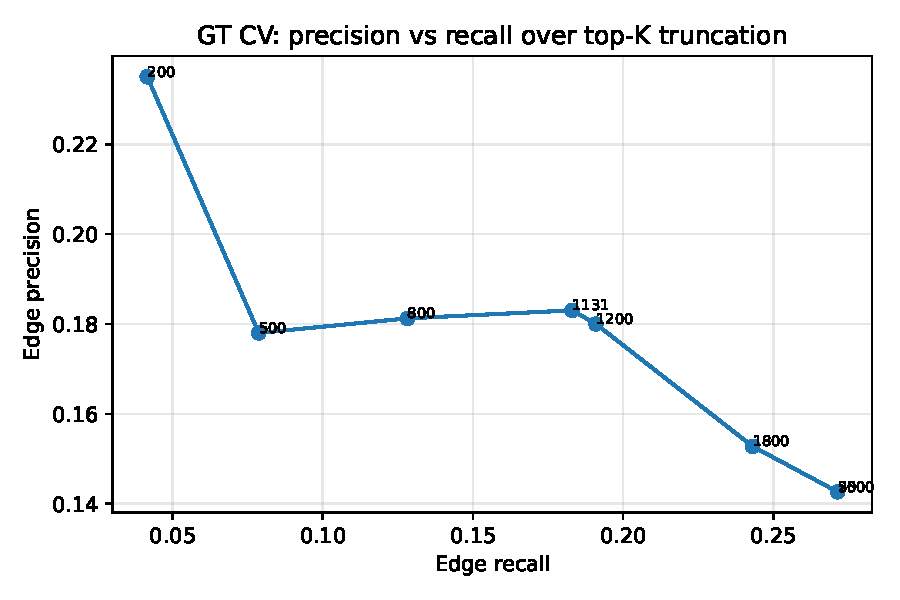
\includegraphics[width=0.82\textwidth]{results/figures/fig_pr_curve.pdf}
\caption{Đường precision--recall khi so sánh \Epre{} train-only với chú giải expert trên Junyi.}
\label{fig:vi-pr}
\end{figure}

Diễn giải hợp lý là đồ thị hành vi và đồ thị chuyên gia nắm bắt hai mặt khác nhau của cấu trúc học tập. Đồ thị hành vi phản ánh các mẫu chuyển tiếp và đồng xuất hiện trong dữ liệu; đồ thị chuyên gia phản ánh thứ tự sư phạm mong muốn. Vì vậy, đồ thị suy luận tự động không nên được tuyên bố là thay thế rẻ cho đồ thị chuyên gia. Khi cả hai nguồn cùng có, hướng mở tự nhiên là mô hình đa quan hệ thay vì chọn một nguồn duy nhất.

\section{Thảo luận và đe dọa hiệu lực}
\paragraph{Ablation null-shift.}
Việc full-log ablation không làm tăng AUC đáng kể không làm yếu yêu cầu kiểm soát rò rỉ. Về phương pháp, thông tin held-out không nên được dùng để dựng feature train, dù shortcut đó có được mô hình khai thác hay không. Kết quả null-shift chủ yếu cho thấy bộ lọc cạnh hiện tại ổn định trên các benchmark lớn.

\paragraph{Tỉa chu trình.}
Trên Junyi, khoảng $47\%$ cạnh ứng viên bị loại trong quá trình phá chu trình. Đây là dấu hiệu dữ liệu hành vi tạo nhiều quan hệ xung đột, không phải bằng chứng pipeline xóa ngẫu nhiên cấu trúc chuyên gia. Heuristic hiện tại loại cạnh yếu nhất trong chu trình; các bản mở rộng nên báo cáo thêm độ nhạy theo mức tỉa.

\paragraph{TBVR.}
TBVR cao trên XES3G5M và Synthetic C2 đo mức trộn tín hiệu trong chính train timeline theo ranh giới kiểm toán nội bộ, không phải lỗi split validation/test. Vì ECR flag bằng $0$, không có bằng chứng người học held-out đi vào train graph.

\paragraph{Giới hạn.}
ASSISTments đã có baseline 3-fold, nhưng Junyi, XES3G5M và các bộ synthetic vẫn dùng fold~0 trong bản phát hành này. Junyi mới bổ sung SKT cache; các mô hình nặng hơn như GKT, GIKT, DyGKT và DGEKT chưa hoàn tất do giới hạn tài nguyên. Wilcoxon với ba fold trên ASSISTments kém mạnh thống kê, nên kết quả significance chỉ nên đọc như kiểm tra minh bạch chứ không phải kết luận cuối cùng.

\section{Kết luận}
Bài báo trình bày một giao thức tái lập để xây dựng và kiểm toán đồ thị \KC{} cho KT dưới ràng buộc kiểm soát rò rỉ. Trên các benchmark công khai, giao thức tạo đồ thị train-only có provenance rõ ràng, đưa đồ thị tiên quyết về DAG, báo cáo trực tiếp các chỉ số rò rỉ, và cho thấy full-log ablation không cải thiện headline AUC ở ba chữ số thập phân. Đối chiếu Junyi cho thấy đồ thị hành vi và đồ thị chuyên gia liên quan ở mức nút nhưng khác đáng kể ở mức cạnh. Các baseline cập nhật nhấn mạnh rằng so sánh mô hình đồ thị với mô hình chuỗi cần báo cáo rõ nguồn gốc cạnh, loại quan hệ, backbone và mức cold-start.

Mục tiêu chính của giao thức không phải chứng minh mô hình đồ thị luôn tốt hơn hoặc tệ hơn mô hình chuỗi, mà là làm cho điều kiện so sánh trở nên kiểm toán được. Khi các cạnh đồ thị trở thành một phần của input mô hình, provenance của chúng phải được xem là thành phần bậc nhất của benchmark.

\bibliographystyle{splncs04}
\bibliography{refs}

\end{document}
